% Doc class required by class assignment.
\documentclass{sig-alternate-05-2015}
\usepackage{graphicx}
% copyright and other misc things provided by template.
% DOI
\doi{10.475/123_4}

% ISBN
\isbn{123-4567-24-567/08/06}

% Conference
\conferenceinfo{PLDI '13}{June 16--19, 2013, Seattle, WA, USA}

\acmPrice{\$15.00}
% end copyright
\begin{document}

% Paper title
\title{WolfTutor
  % \titlenote{(Paper 1). For use with
  % SIG-ALTERNATE.CLS. Supported by ACM.}
}
\subtitle{A system to enable peer tutoring built on Slack
  % \titlenote{A full version of this paper is available as
  % \textit{Author's Guide to Preparing ACM SIG Proceedings Using
  % \LaTeX$2_\epsilon$\ and BibTeX} at
  % \texttt{www.acm.org/eaddress.htm}
  % }
}

\numberofauthors{4} %  in this sample file, there are a *total*
\author{
  \alignauthor
  {Monica Metro}\\
  \affaddr{North Carolina State University}\\
  \affaddr{3021 F Dorner Circle}\\
  \affaddr{Raleigh, NC}\\
  \email{mgmetro@ncsu.edu}
  % 2nd. author
  \alignauthor
  {Zachery DeLong}\\
  \affaddr{North Carolina State University}\\
  \affaddr{2305 Horizon Hike Ct}\\
  \affaddr{Raleigh, NC}\\
  \email{zpdelong@ncsu.edu }
  % 3rd. author
  \alignauthor 
  {Zhangqi Zha} \\
  \affaddr{North Carolina State University}\\
  \affaddr{1800 Vienna Wood Dr}\\
  \affaddr{Raleigh, NC}\\
  \email{zzha@ncsu.edu}
}
% Generate page header.
\maketitle

% Paper body
\begin{abstract}
In this abstract, we need to preview our experiment and our results 
\end{abstract}
%%% Local Variables:
%%% mode: latex
%%% TeX-master: "../main"
%%% End:


\section{Introduction}
\label{sec:intro}
\subsection{What is WolfTutor}
\label{sec:what-wolftutor}

\subsection{WolfTutor Use Cases}
\label{sec:wolftutor-use-cases}

\subsection{Pain Points with Wolf Tutor}
\label{sec:pain-points-with}

\subsection{Initial Study}
\label{sec:initial-study}

%%% Local Variables:
%%% mode: latex
%%% TeX-master: "../../main"
%%% End:


\section{Enhancements}
\label{sec:enhancements}


\subsection{Pain Points}
\label{sec:pain-points} The original creators of WolfTutor proposed
three additional features for future development. The first was to
integrate an online platform to conduct tutoring sessions online. The
second was to allow both the tutor and the student to sync their
session reservation with their calendar, e.g. Google Calendar. Lastly,
to update the scheduling algorithm such that a user could edit or
delete reservations in addition to being able to create and view
them. Our team provided two other features: increasing matching
options between tutors and students and allowing students to browse
their reservation history.

After careful consideration, three main pain points were decided upon
that consisted of the proposed enhancements. Integration of an online
platform was discarded because it was not thought to facilitate the
quality of the match between tutor and student.

\paragraph{Scheduling and Calendar Sync} WolfTutor currently only
allows users seeking a tutoring session to create and view
reservations. In real life, people change their mind or events come up
such that a schedule change is in order. The ability to cancel or
reschedule reservations would make WolfTutor more applicable to real
world scheduling scenarios. In addition, facilitating intergration
with commonly used calendars such as Google and IOS Calendar extends
this principle of making scheduling easier.

\paragraph{Increasing Matching Options} In regards to matching with
tutors, WolfTutor currently displays a list of tutor's and their
ratings based on the student's desired subject. Then, the student may
attempt to book a reservation with a tutor they choose. By expanding
matching options, a student should be able easily find a higher
quality match with a tutor. For example, a student could filter tutors
by location by selecting only locations they want to meet up at in a
checkbox. Similarily, if a student has a few tutors they prefer, they
could select those names from a checkbox such that WolfTutor only
displays those tutors. This type of filtering system is often used by
medical facilities with multiple practioners and multiple practing
sites. It is also used by NC State University's scheduling tool on
epack.

\paragraph{History and Recommendations} WolfTutor does currently allow
for student's to review and rate the tutors that they met with
previously. However, there is no way to view a student's reservation
history past the most recent tutor. WolfTutor also does not provide a
way for a student to easily re-book a new reserveration with a tutor
they chose previously if they liked the tutor and would like to
schedule a reservation with them again. Adding these enhancements
would increase ease of use by helping a student distinguish between a
competent and non-competent tutor they've had in the past.

\subsection{Initial Study}
\label{sec:initial-study} A survey was conducted to determine which
enhancement the intended user base (students) prefered the most. The
survey was separated into three parts.

\paragraph{Background} A background section measured how prevalent
scheduling was within the daily life of the participants. Most
participants admitted having to schedule a meeting within the last
year.

\paragraph{Priorities} The next section revealed which enhancement the
participants thought was a priority by asking them to rate the level
of important the enhancement was on a scale from 1 (least important)
to 5 (most important). To avoid bias, instead of explaining the
enhancements out, the survey questions were created around the base
point of the enhancement:
\begin{itemize}
  \item "When scheduling a tutoring meeting, picking the location is
very important to me."
  \item "When scheduling a tutoring meeting, the competency of the
tutor is very important to me."
  \item "When scheduling a tutoring meeting, being able to agree on a
time quickly and easily is very important to me."
\end{itemize} The question regarding competency scored the highest
level of important among the participants collectively. Scheduling and
increased matching (by location) followed respectively.

\paragraph{Trade Offs} The objective of the third section was to
validiate the results in the second section by asking the participants
which enhancements they would be willing to compromise on in order to
get the enhancement they thought was more important. The questions
included:
\begin{itemize}
  \item "When scheduling a tutoring meeting, I am willing to make
trade-offs on the competency of the tutor and time if I can specify
the location of the meeting."
  \item "When scheduling a tutoring meeting, I am willing to make
trade-offs on location and time if I can specify the competency of my
tutor."
  \item "When scheduling a tutoring meeting, I am willing to make
trade-offs in location and competency if I can specify the time of the
meeting."
\end{itemize} Again, competency scored the highest as the most
important enhancement collectively. Scheduling followed in second
place and location matching in third.

\paragraph{Other} An option was given to participants to suggest a new
enhancement. The only received response was to integrate the
application with Skype.

\subsection{Chosen Enhancement}
\label{sec:chosen-enhancement}
% What do we want to do?
% - what is the goal?
% - Why is that our goal?
% - What do we propose?
% - Why does that solve the problem we are setting out to solve?

Given the surveying discussed above, it seems clear that what students
in our class want is a way to more easily match with competent
tutors.  To that end, WolfTutor currenly does very little in terms of
matching.  It provides students with the ratings of the available
tutors, which is a good first step, but it does nothing to help
organize the available tutors and prioritize them to make searching
sutdents' lives easier.  

WolfTutor also has a significant amount of data about a student's
history with their tutors, but it does fairly little with that
information.  To help improve matching between students and tutors, we
propose to use that historical data during the matching process. To do
that, we will implement a suggestion algorithm that will pull out the
students' previous interactions and use their positive reviews to push
certain tutors higher in the list and their negative reviews to push
other tutors lower on the list.

One problem with this approach is that it discourages students from
matching with new tutors, because their lack of history will push them
further down on the list.  In the interests of helpign alleviate this
problem, a third dimension should be added to the suggestion
algorithm: the interactions from students to tutors.  In the proposed
model, the ratings of tutors and students and the ratings of the
current student to the tutor in quesiton are the major focus of the
algorithm, but no consideration is given to the interactions of
students with their tutors.  This new third dimension should encourage
tutors who have already tutored a new tutor in the past (and had a
positive experience with them) to match.  This should help both
encourage students who have used the platform as students to convert
to tutors, and it should also help give those students who do convert
a leg up in being found by students to tutor.

This will hopefully make it easier for students to match with not only
tutors that are well reviewed and rate well in the subjects they are
interested in, but also encourage students to build longer-term
mentoring relationships with tutors that work well with them.  

Next we will discuss the application's architecture in section
\ref{sec:architecture} and the evaluation plan for this idea \ref{sec:validation}.
%%% Local Variables:
%%% mode: latex
%%% TeX-master: "../../../main"
%%% End:


%%% Local Variables: %%% mode: latex %%% TeX-master: "../../main" %%%

\section{Architecture}
\label{sec:architecture}
% \subsection{Original Architecture}
\label{sec:Original-Architecture}
This section outlines the various components of the system and how they interact with one and another. The detailed architecture is described in figure \ref{sec:architecture:fig:O-Architecture}.

\begin{figure*}[ht]
\label{sec:architecture:fig:O-Architecture}
\caption{Original Architecture Design}
\centering
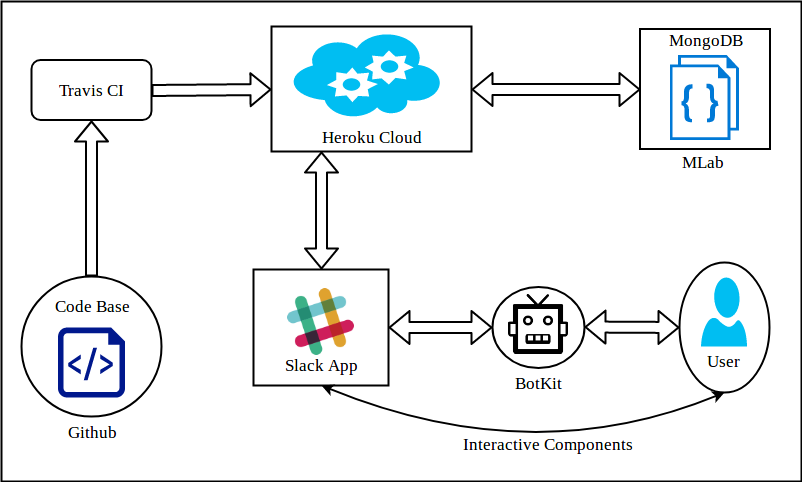
\includegraphics[width=\textwidth]{O-Architecture.png}
\end{figure*}

Broadly speaking, the architecture is divided in three main components: the slack app, the heroku cloud and the mongoDB database. This separation of concerns is a major advantage since database is independently hosted on mlab server and can be accessed from anywhere with valid authorization credentials. The heroku cloud hosts the logic of the slack app, which communicates with the user. The system also implemented the continuous deployment, continuous integration pipeline with Travis CI, which directly pushes the code to heroku cloud once the build passes (also indicated in the readme section of the repository). The test cases was also generated which acts as a sanity check for any commit made to the master branch, before deployment so as to not push broken code on the production server at heroku. Following is the detailed description of each component of the architecture.

\paragraph{Slack App}
Slack App is generated in api.slack.com dashboard. It is currently developed only for one workspace and it is configured to communicate to the heroku server which is hosted at wolftutor.herokuapp.com. Also creating a slack app gives us various authentication tokens like access token and verification token which are required for Slack to authorize that the requests and responses are coming from a valid production server. Slack app also gives us configuration of the bot like its name its icon, etc. This will be visible to the user when the user interacts with the bot. Slack bot is a part of the slack app, where bot is considered like a user (bot-user) in slack terminology. Slack app also allows access to interactive components like dialogs and message menus for the overall user experience to be more rich and interesting.

\paragraph{BotKit}
Botkit is an external library that integrates with Realtime API which can detect patterns in the user queries. The logic to be executed when a particular pattern is detected is written in the slack app (NodeJS code hosted on heroku). For instance, on saying hi user should be given an option to enroll in the system. This is one example of working of the Botkit module.

\paragraph{Code Base}
Code base is the Github repository where we maintain our code. Following the general convention, we made new branch for every new logical feature and also linked issues with particular merge commits. All this activity can be viewed in our repository. We have also used conventional practises of separating database queries and put them all together in model directory. Also all of our interactive components are in distributed in different folders.

\paragraph{Continuous Integration Module}
The master branch of our repository is linked with Travis CI to be pushed to heroku server if the build on travis CI passes. The tests written in mocha acts as a final sanity check before deploying the code on the production server. Any code that is pushed on the master is directly built on Travis CI and deployed on heroku server if build passes.

\paragraph{Heroku Server}
Heroku server is the home of our NodeJS application. We have used single dyno (free version) to host the application. The code pushed on master is deployed here by Travis and we always have the latest code in the production server. Also we have included the Procfile where it is indicated what command to execute to run the application (npm start). This is necessary for heroku to understand the starting point of the application.

\paragraph{Database}
Mlab is a server that hosts our Mongo Database. The advantage of having a remote server for mlab is that everyone can access the same data at simultaneously. In mongo, only a mongo URI is required for accessing the database along with valid user credentials. This makes it very simple to test the application locally as well as run in on the server.

\paragraph{User}
User is anyone who is signed in into the Slack workspace where the slack app is added. He/She can communicate with the app in variety of ways as described in the use-cases section. Also he/she can interact with the app using dialogs and message drop-downs and buttons to give a particular command. See details in use-cases section.

% \paragraph{
%%% Local Variables:
%%% mode: latex
%%% TeX-master: "../../../main"
%%% End:



%%% Local Variables:
%%% mode: latex
%%% TeX-master: "../../main"
%%% End:


\section{Progress}
\label{sec:progress}
% Based on the experience of previous project, the team chose the spiral model
of software development methodologies. A spiral model is a form of 
risk-driven development where the most risky parts of a project are 
identified early and planned into prototypes that can inform the final 
product. See the breakdown of the prototypes the team chose in table \ref{sec:progress:prototypes-table}.

\begin{table*}[!htbp]
\caption{Prototypes and Schedules}
\label{sec:progress:prototypes-table}
\begin{center}
\begin{tabular}{  l  l p{10cm} }
	\bf Schedules & \bf Prototypes/Work & \bf Descriptions\\ \hline \\
	Week 1 & Planning and Pre-survey & Get the original project to work, plan a few changes and enhacenments, do a user survey\\
	Week 2 & Project Proposal & Detail the plan and get ready the project proposal\\
	Week 3-1 & Prototype 1 & Gernerate dummy data, build loading history interface\\
	Week 3-2 & Prototype 2 & Gernerate dummy data, build suggestion interface\\
	Week 4-1 & Prototype 3 & Build suggestion algorithm and intergated into final system \\
	Week 4-2 & Prototype 4 & System evaluation, user testing, update system \\
	Week 5 & Presentation & Present the final system \\
	Week 6/7 & Final Paper & Draft and finalize the paper \\
\end{tabular}
\end{center}
\end{table*}


This afforded the team the ability to have regular check-ins and to measure
progress against the prototypes. The team will convene two to three times 
a week to do pair programming and to check progress against the prototypes.
When combined with regular check-ins with the TAs, the team shall be able 
to build prototype programs to perform design feature and functionality.

We also used Gitup project boards to create and track our progress. This 
method featured the ability to send a notification to the team member to 
remind and collaborate within the team members. Here is the example image.

\begin{table}[ht]
\caption{Progress Tracking Board}
\label{section:progress:tracking-board}
\centering
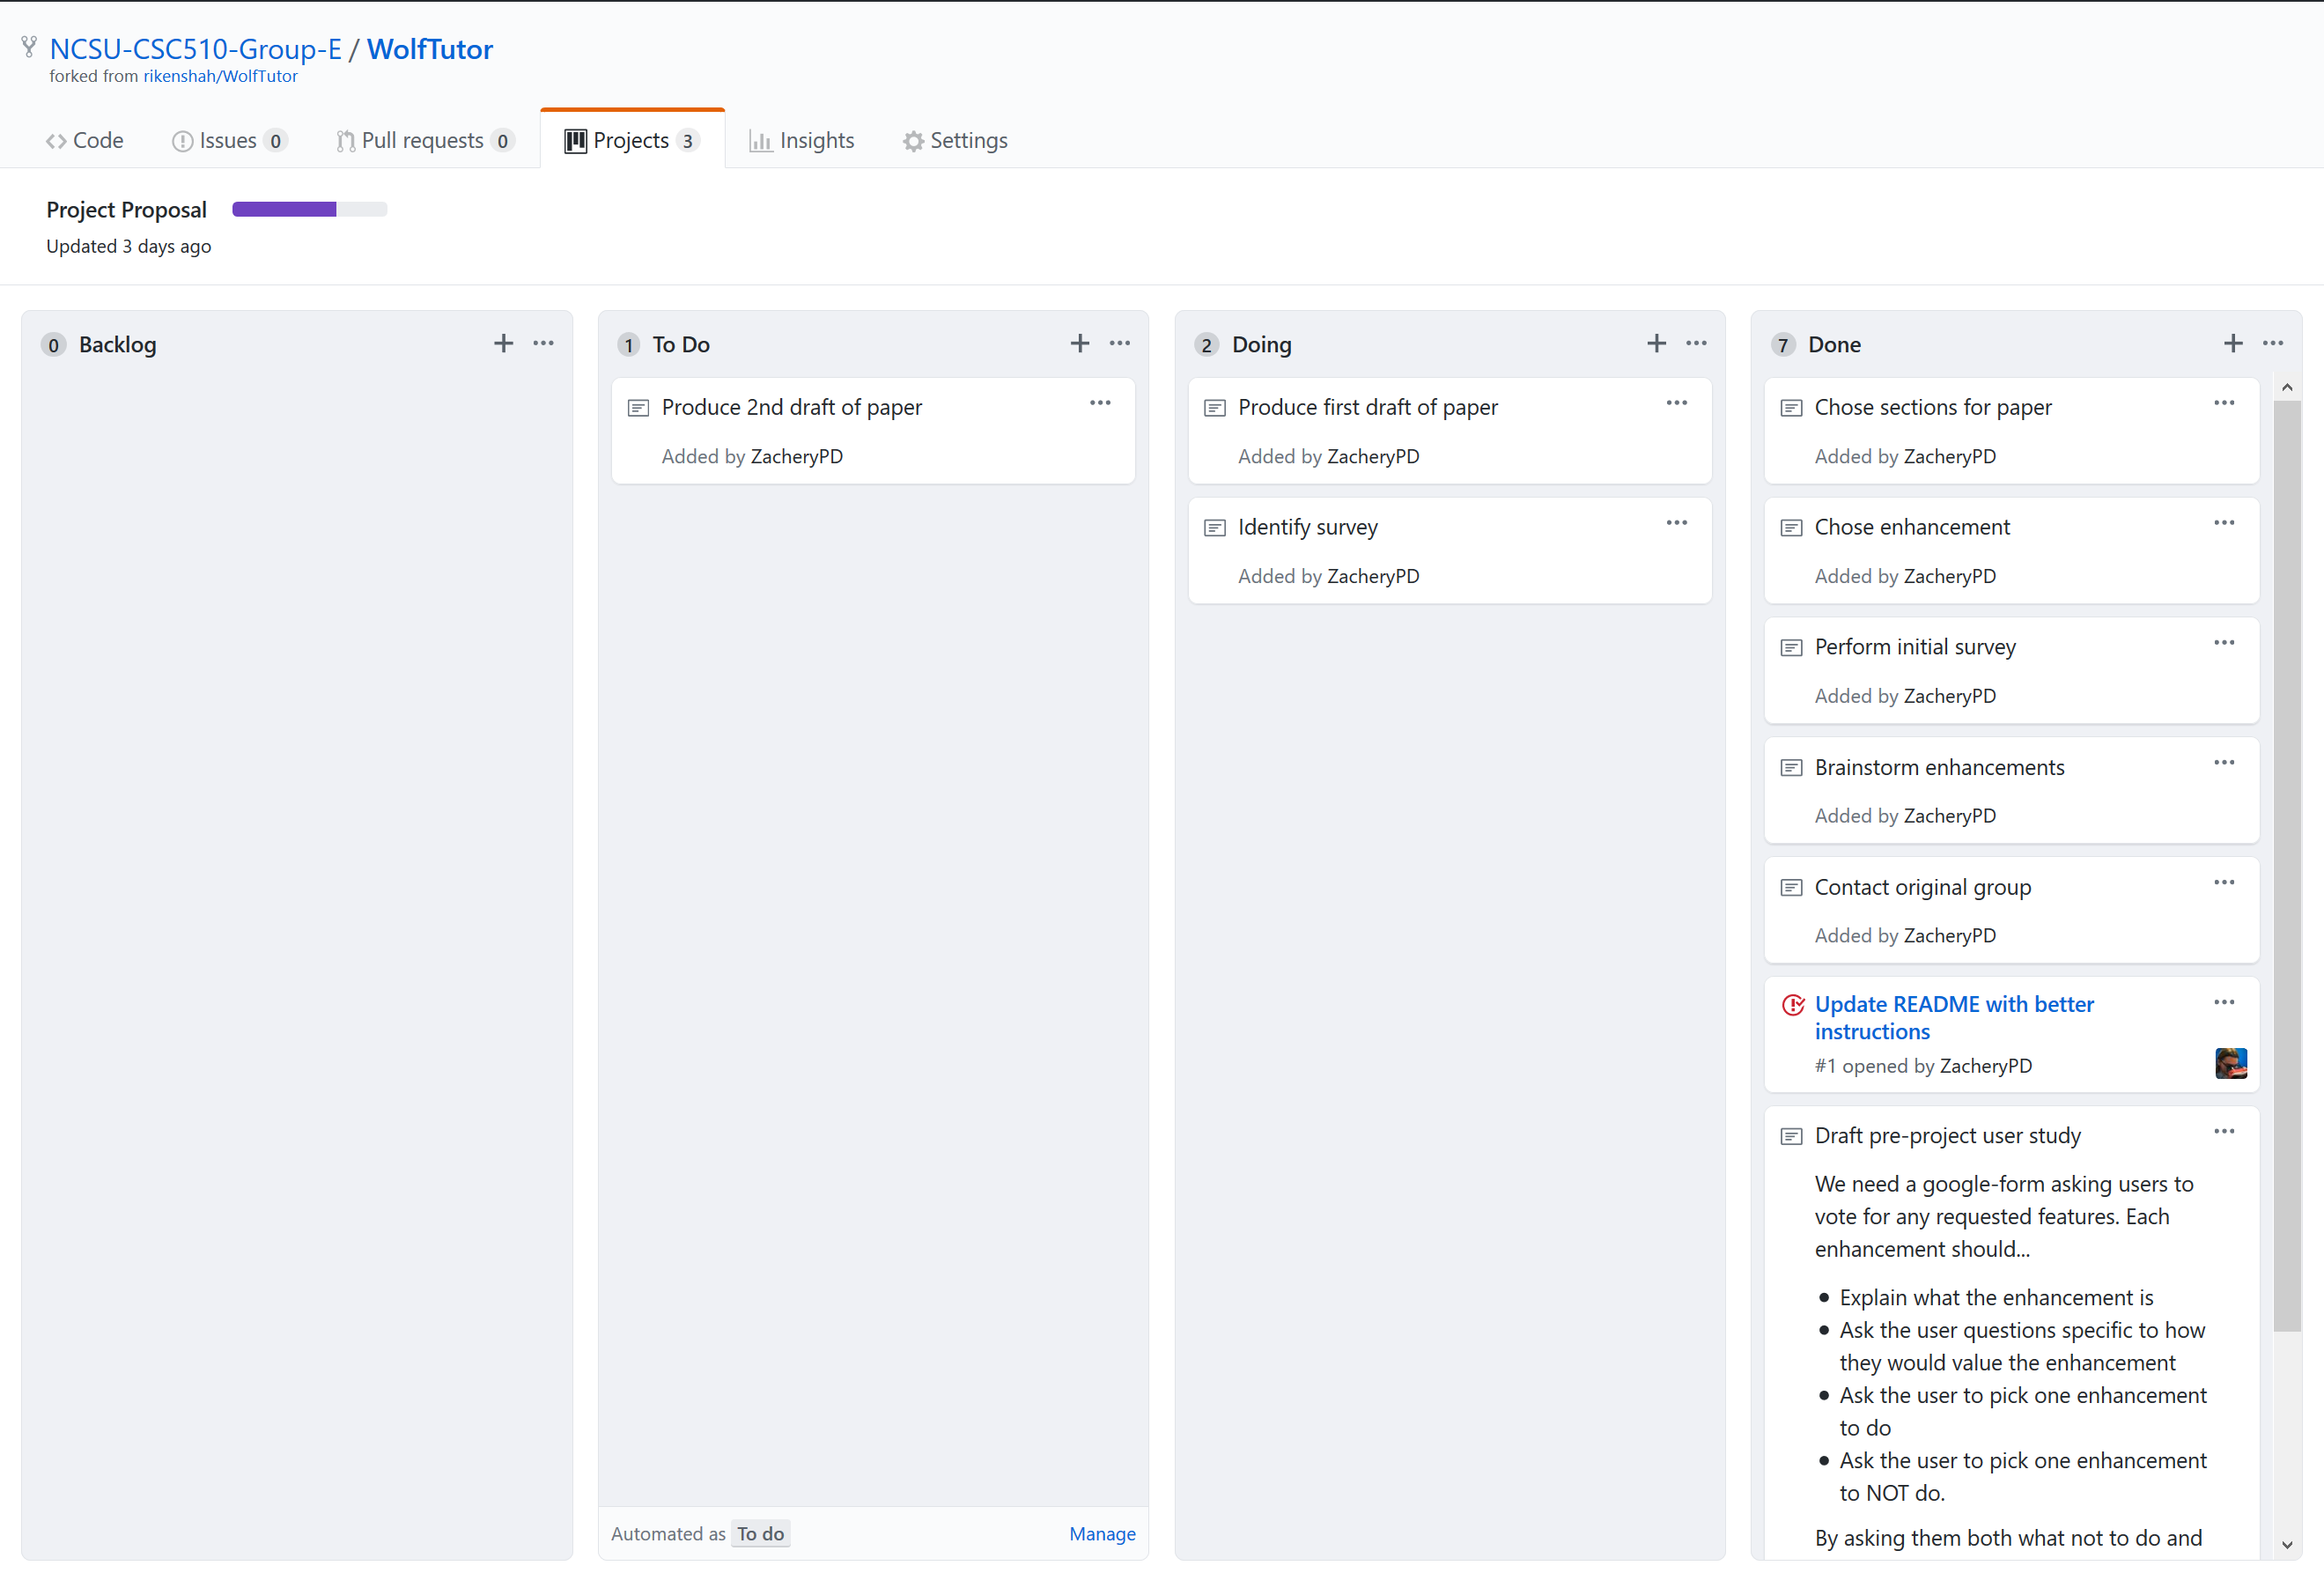
\includegraphics[width=0.48\textwidth]{progress.png}
\end{table}

\section{Validation}
\label{sec:validation}
% % What do we want to evaluate
% Why do we want to evaluate that?

\subsection{Evaluating Matching}
\label{sec:evaluating-matching}
% How?
% Process?
% Data?


\subsection{Evaluating Usability}
\label{sec:evaluating-usability}
% How
% When
% Data?


%%% Local Variables:
%%% mode: latex
%%% TeX-master: "../../main"
%%% End:


\section{Conclusion}
\label{sec:conclusion}

\subsection{Schedule}
\label{sec:schedule}
% % Please do not delete!  thanks! -- zach
% !TEX root = ../main.tex


\subsection{Future enhancement}
During our initial brainstorming and pre-survey mentioned in section \ref{sec:enhancements}, several possible enhancements were discussed. The addition of optional filters to facilitate more specific matching when searching for a tutor, integtration with commonly used online calendar applications to facilitate booking a slot and to increase ease of use, the ability to cancel or reschedule a reservaton, allowing a student to view their reservation history and to use their history to make better recommendations for their next tutor, and integrating an online video interface to conduct tutoring sessions. Considering the short time frame for the project, we chose to implement the feature that was rated as the most important by our intended audience: viewing reservation history and giving recommendations for tutors with the goal of recommending a tutor the student would rate highly. The other features will be considered as future enhancements.


% REMOVE NOCITE OR IT WILL LIST EVERYTHING IN YOUR DATABASE AS A REFERENCE
% \nocite{*}

% Bibliography/style
\bibliographystyle{abbrv}

\bibliography{export}
% End bibliography/style

\end{document}
